\begin{enumerate}[label=\arabic*.,ref=\theenumi]
%		\numberwithin{figure}{enumi}
\item Obtain the Boolean Expression for the Logic circuit shown below
in \figref{fig:2013/c/6/b}.
\label{prob:2013/c/6/b}
\hfill (CBSE 2013)
	\usetikzlibrary{circuits.logic.IEC,calc}
		\begin{figure}[!ht]
\centering
	   \begin{circuitikz} \draw
(0,2) node[or port]  (myor1) {}
(0,0) node[and port] (myand) {}
(2,1) node[or port] (myor2) {}
(myor1.out) -- (myor2.in 1)
(myand.out) -- (myor2.in 2);

\node[left] at (myor1.in 1) {\(X\)};
\node[left] at (myor1.in 2) {\(Y\)};
\node[left] at (myor1.in 1)[ocirc] {};
\node[left] at (myand.in 2) [ocirc] {};
\node[left] at (myand.in 1) {\(Y\)};
\node[left] at (myand.in 2) {\(Z\)};
\node[right] at (myor1.out) {};
\node[right] at (myand.out) {};

\node[right] at (myor2.out) {F};
\end{circuitikz}
			\caption{}
\label{fig:2013/c/6/b}
		\end{figure}
\item Verify the Boolean Expression 
\label{prob:2013/c/6/a}
\hfill (CBSE 2013)
		\begin{align}
\label{eq:2013/c/6/a}
	               A+C=A+A'C+BC
		\end{align}
\item Draw the Logic Circuit for the following Boolean Expression 
\hfill (CBSE 2015)
\label{prob:2015-1/c/6/b}
		\begin{align}
\label{eq:2015-1/c/6/b}
f(x,y,z,w) = (x'+y)z + w'
		\end{align}
\item Verify the following
\hfill (CBSE 2015)
\label{prob:2015-1/c/6/a}
		\begin{align}
\label{eq:2015-1/c/6/a}
U' + V = U'V' + U'V+UV
		\end{align}
\item Draw the Logic Circuit for the given Boolean Expression
\hfill (CBSE 2015)
\label{prob:2015/c/6/b}
		\begin{align}
\label{eq:2015/c/6/b}
(U + V')W' + Z
		\end{align}
\item 
Verify the following using Boolean Laws
\label{prob:2015/c/6/a}
\hfill (CBSE 2015)
		\begin{align}
\label{eq:2015/c/6/a}
X+Y' = XY+XY'+X'Y'
		\end{align}
\item 
\label{prob:2016/c/6/b}
Write the Boolean Expression for the result of the Logic Circuit as shown in Fig.  
\ref{fig:2016/c/6/b}
\hfill (CBSE 2016)
\begin{figure}
\centering
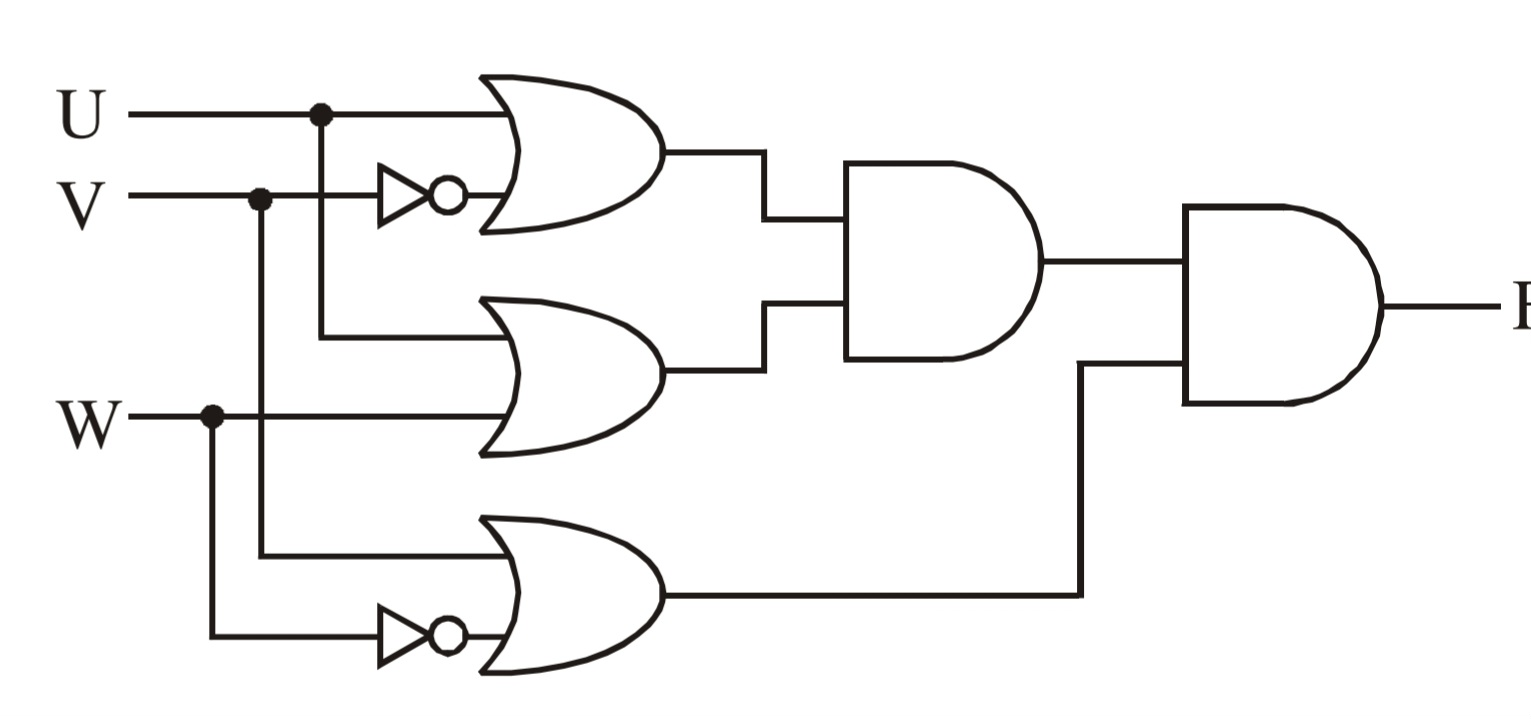
\includegraphics[width=\columnwidth]{figs/cbse-2016.jpg}
\caption{}
\label{fig:2016/c/6/b}
\end{figure}
\item Draw the logic circuit of the following Boolean Expression using only NAND Gates.
\hfill (CBSE 2017)
\label{prob:2017-1/c/6/b}
		\begin{align}
\label{eq:2017-1/c/6/b}
 XY + YZ
		\end{align}
\item Draw the Logic Circuit of the following Boolean Expression using only NOR Gates  
\hfill (CBSE 2017)
\label{prob:2017/c/6/b}
      \begin{align}
      (A+B)(C+D)
      \end{align}
\item Draw the Logic Circuit of the following Boolean Expression
\hfill (CBSE 2018)
\label{prob:2018/c/6/b}
\begin{equation} 
(U'+V)(V'+W')
\end{equation}
\item Derive a Canonical POS expression for a Boolean function F, represented by 
Table \ref{tab:2019/c/6/c}\hfill (CBSE 2019)
\label{prob:2019/c/6/c}
\begin{table}[!ht]
\centering
\begin{tabular}{|l|l|l|c|}
	\hline
	X&Y&Z&F(X,Y,Z)\\
	\hline
	0&0&0&1\\
	0&0&1&0\\
	0&1&0&1\\
	0&1&1&0\\
	1&0&0&1\\
	1&0&1&1\\
	1&1&0&0\\
	1&1&1&0\\
	\hline
\end{tabular}
\caption{}
\label{tab:2019/c/6/c}
\end{table}
\item For the logic circuit shown in \figref{fig:2000/gate/ec/2/7}, find the simplified Boolean expression for the output. 
\label{prob:2000/gate/ec/2/7}
\hfill (GATE EC 2000)
\begin{figure}[!ht]
    \centering
    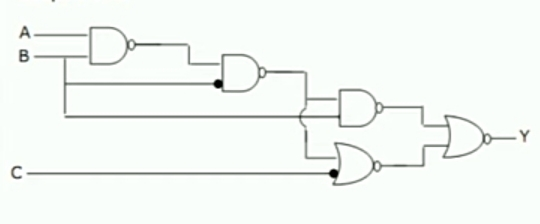
\includegraphics[width=\columnwidth]{figs/2000-gate-ec-2-7.jpg}
    \caption{}
\label{fig:2000/gate/ec/2/7}
\end{figure}
\item 
Obtain the Boolean Expression for the Logic circuit shown below
in \figref{fig:1993/gate/ec/4/8}.
\label{prob:1993/gate/ec/4/8}
\hfill (GATE EC 1993)
\begin{figure}[!ht]
    \centering
    \resizebox{\columnwidth}{!}{%
	   \begin{circuitikz} \draw
(0,2) node[nand port] (mynand1) {}
(2,3) node[nand port] (mynand2) {}
(0,0) node[nand port] (mynand) {}
(2,-1) node[nand port] (mynand3) {}
(2,1) node[or port] (myor1) {}
(4,1) node[or port,number inputs =3] (myor2) {}
(mynand1.out) -- (myor1.in 1)
(mynand.out) -- (myor1.in 2)
(mynand2.out) -- (myor2.in 1)
(mynand3.out) -- (myor2.in 3)
(myor1.out) -- (myor2.in 2);
\node[left] at (mynand1.in 1) {\(A\)};
\node[left] at (mynand1.in 2) {\(B\)};
\node[left] at (mynand2.in 1) {\(A\)};
\node[left] at (mynand2.in 2) {\(A\)};
\node[left] at (mynand3.in 1) {\(C\)};
\node[left] at (mynand3.in 2) {\(C\)};
\node[left] at (mynand1.in 1)[ocirc] {};
\node[left] at (mynand.in 2) [ocirc] {};
\node[left] at (mynand.in 1) {\(B\)};
\node[left] at (mynand.in 2) {\(C\)};
\node[right] at (mynand1.out) {};
\node[right] at (mynand.out) {};
\node[right] at (mynand2.out) {};
\node[right] at (mynand3.out) {};
\node[right] at (myor2.out) {\(Y\)};
\end{circuitikz}
	}
    \caption{}
\label{fig:1993/gate/ec/4/8}
\end{figure}
%
\item Implement Table
\ref{tab:1993/gate/ec/6/13}
using XNOR logic.
\hfill (GATE EC 1993)
\label{prob:1993/gate/ec/6/13}
\begin{table}[!ht]
	\centering
	\begin{tabular}{|c|c|c|}
		\hline
		\textbf{A}&\textbf{B}&\textbf{Y}\\
		\hline
		0&0&1\\
		\hline
		0&1&0\\
		\hline
		1&0&0\\
		\hline
		1&1&1\\   
		\hline 
	\end{tabular}
	\caption{}
\label{tab:1993/gate/ec/6/13}
\end{table}
\item 
\label{prob:1999-gate-ec-2-11}
For a binary half-sub-tractor having two inputs A and B, find the correct set of logical expressions for the outputs D (=A minus B) and X (=borrow).
\hfill (GATE EC 1999)
%
\item 
Find $X$ in the following circuit in 
\figref{fig:2007-gate-ec-43}
\hfill (GATE EC 2007)
\label{prob:2007-gate-ec-43}
\begin{figure}[!ht]
\centering
	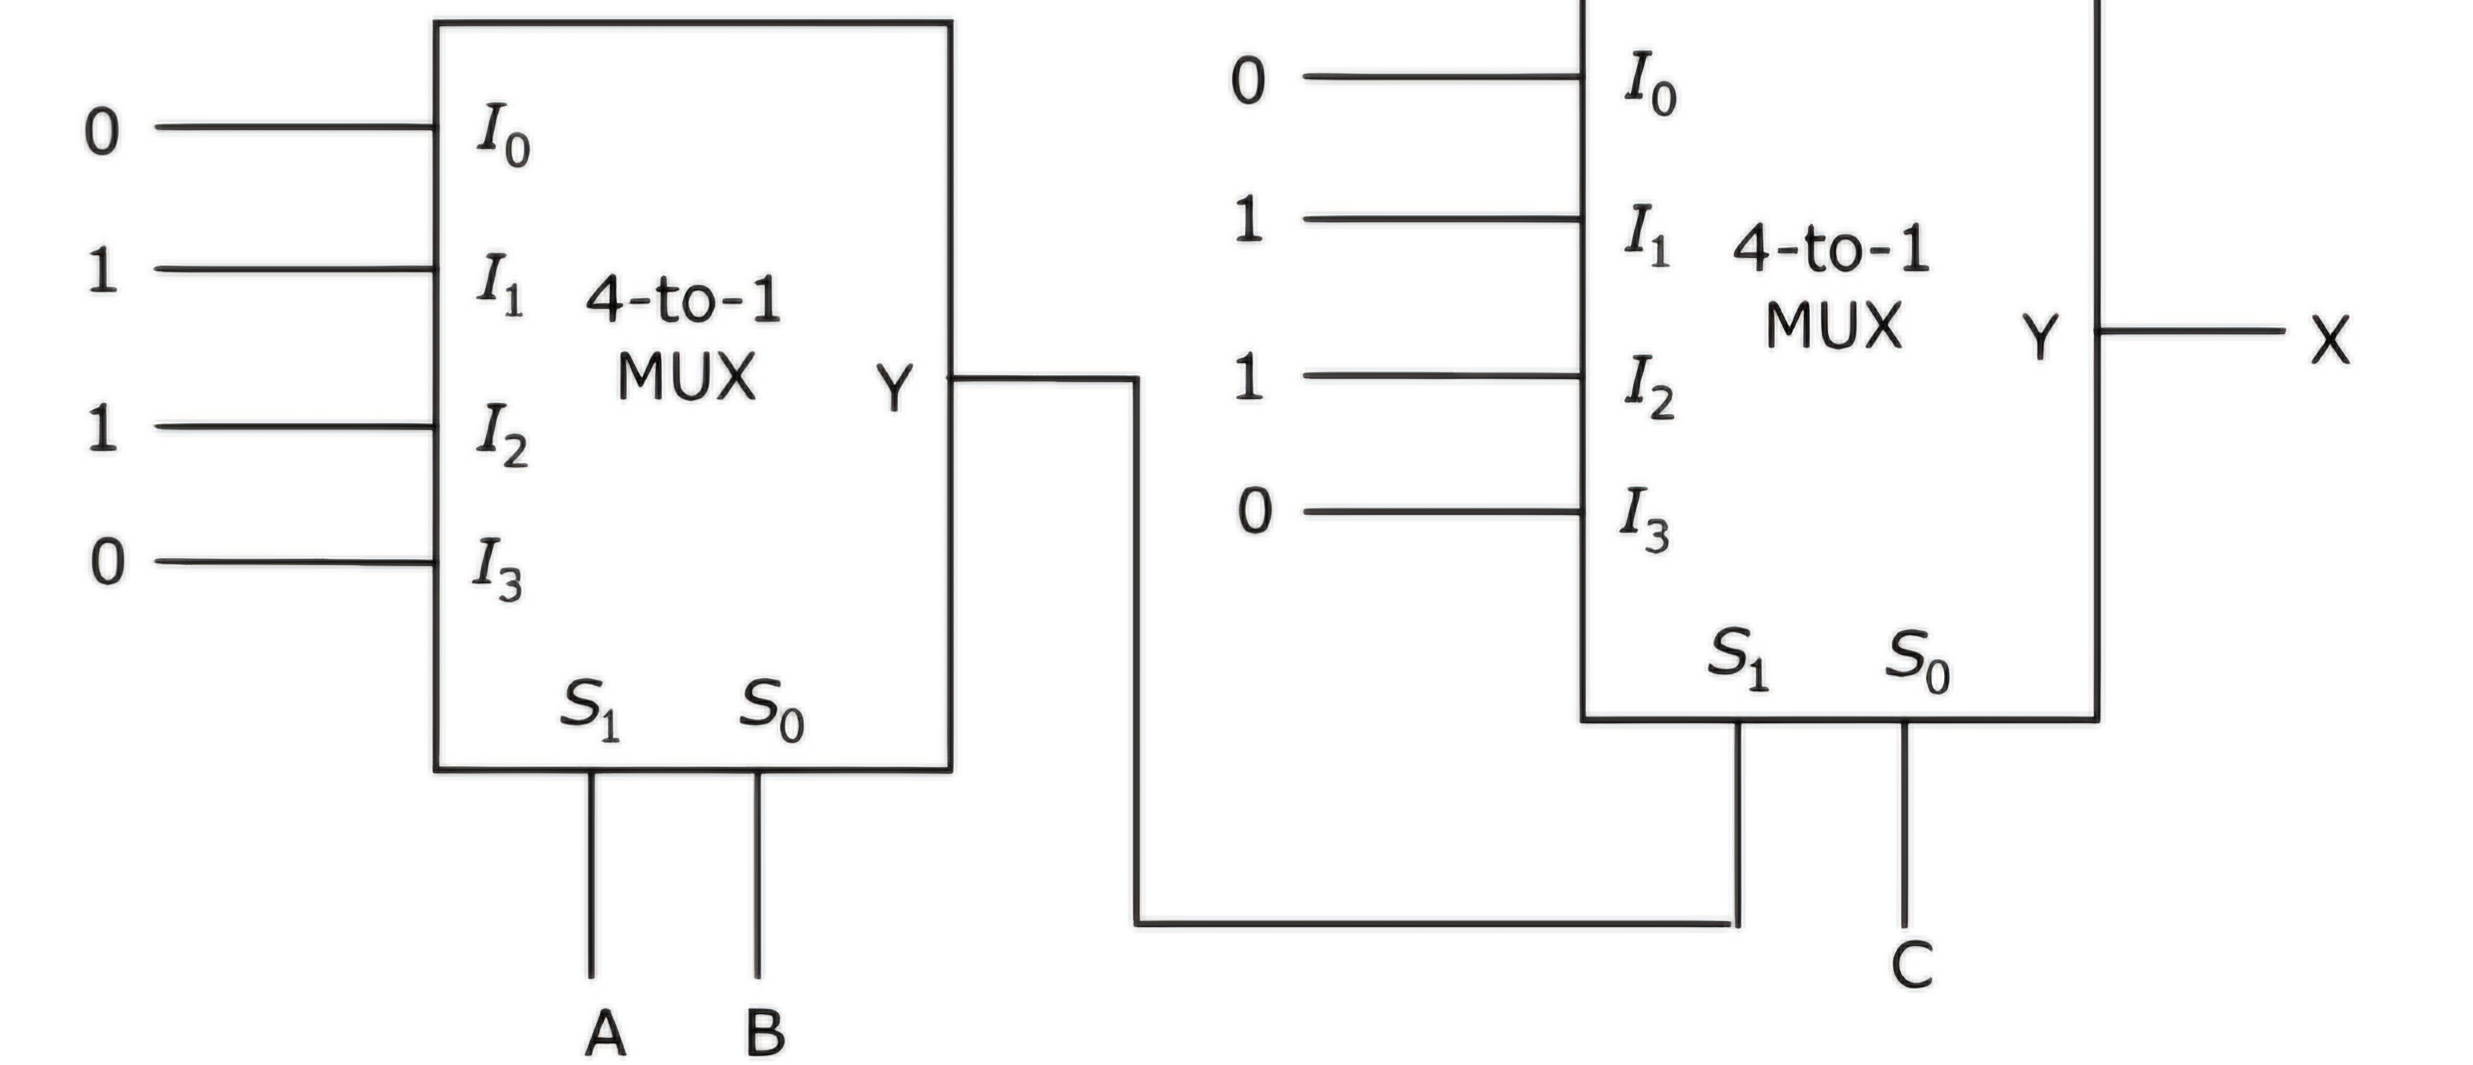
\includegraphics[width=1\columnwidth]{figs/2007-gate-ec-43.png}
\caption{}
\label{fig:2007-gate-ec-43}
\end{figure}
\item 
\label{prob:2007-gate-in-10}
      A logic circuit implements the boolean function F=X'.Y+X.Y'.Z'. It is found that the input combination X=Y=1 can never occur. Taking this into account, find a simplified expression for F. 
\hfill (GATE IN 2007)
\item 
\label{prob:2010-gate-ec-39}
Find the Boolean logic realised by the following circuit in 
\figref{fig:2010-gate-ec-39}
\hfill (GATE EC 2010)
\begin{figure}[!ht]
\centering
	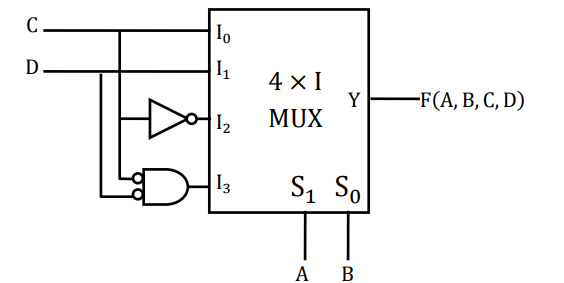
\includegraphics[width=1\columnwidth]{figs/2010-gate-ec-39.png}
\caption{}
\label{fig:2010-gate-ec-39}
\end{figure}
\item 
\label{prob:2011-gate-ec-20}
Find the logic function implemented by the circuit given below 
in 
\figref{fig:2011-gate-ec-20}
\hfill (GATE EC 2011)
\begin{figure}[!ht]
\centering
	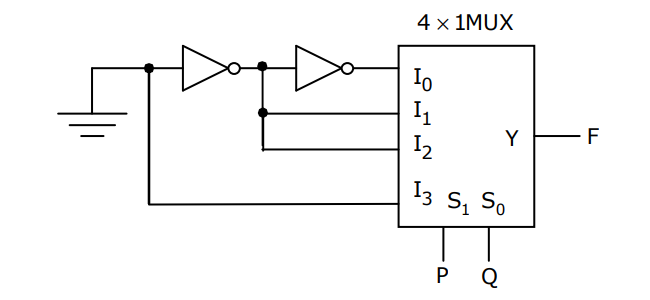
\includegraphics[width=\columnwidth]{figs/2011-gate-ec-20.png}
\caption{}
\label{fig:2011-gate-ec-20}
\end{figure}
\item
\label{prob:2016/gate/in/19}
Find F in the Digital Circuit given in the figure below
in \figref{fig:2016/gate/in/19}.
\hfill (GATE IN 2016)
\begin{figure}[!ht]
	\centering
	\resizebox{\columnwidth}{!}{%
\begin{tikzpicture}
 

 
% Logic ports
\node[nand port] (a) at (2,1){};
\node[nand port] (b) at (2,4){};
\node[nand port] (c) at (4,0){};
\node[nand port] (d) at (6,3){};

 
% Connection

 
\draw (a.in 2) -| (b.in 2);
\draw (b.out) -| (d.in 1);
 
\draw (a.out) -|  (c.in 1);
\draw (c.out) -| (d.in 2);
\draw (d.out) -- ++(1,0) node[near end,above]{F};
 
\draw (b.in 1) -- ++(-1.5,0)node[left](In1){X};
\draw (b.in 2) -- ++(-1.5,0)node[left](In3){Y};
\draw (c.in 2) -- ++(-1.5,0)node[left](In3){Z};
% Jump crossing element
1
\end{tikzpicture}
	}
	\caption{}
\label{fig:2016/gate/in/19}
\end{figure}


\item 
\label{prob:2017-gate-ec-16}
Find the logic function implemented by the circuit given below 
in 
\figref{fig:2017-gate-ec-16}
\hfill (GATE EC 2017)
\begin{figure}[!ht]
\centering
	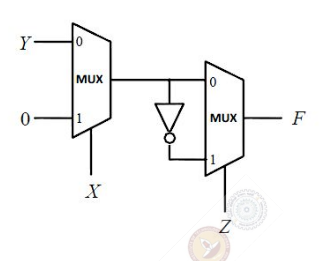
\includegraphics[width=\columnwidth]{figs/2017-gate-ec-16.png}
\caption{}
\label{fig:2017-gate-ec-16}
\end{figure}
\item 
\label{prob:2018-gate-ec-31}
Find the logic function implemented by the circuit given below 
in 
\figref{fig:2018-gate-ec-31}
\hfill (GATE EC 2018)
\begin{figure}[!ht]
\centering
	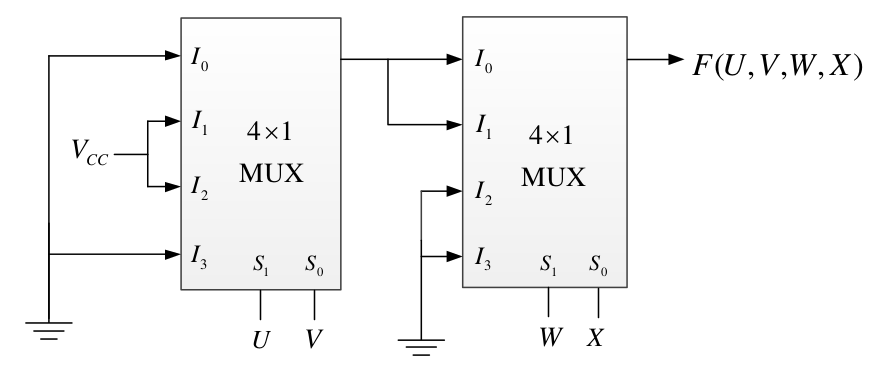
\includegraphics[width=\columnwidth]{figs/2018-gate-ec-31.png}
\caption{}
\label{fig:2018-gate-ec-31}
\end{figure}
\item 
\label{prob:2018-gate-ee-14}
Find the logic function implemented by the circuit given below 
in 
\figref{fig:2018-gate-ee-14}
\hfill (GATE EE 2018)
\begin{figure}[!ht]
\centering
	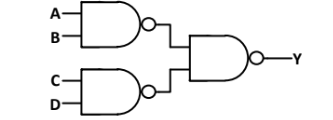
\includegraphics[width=\columnwidth]{figs/2018-gate-ee-14.png}
\caption{}
\label{fig:2018-gate-ee-14}
\end{figure}
\item 
\label{prob:2019-gate-ee-36}
Find the logic function implemented by the circuit given below 
in 
\figref{fig:2019-gate-ee-36}
\hfill (GATE EE 2019)
\begin{figure}[!ht]
\centering
	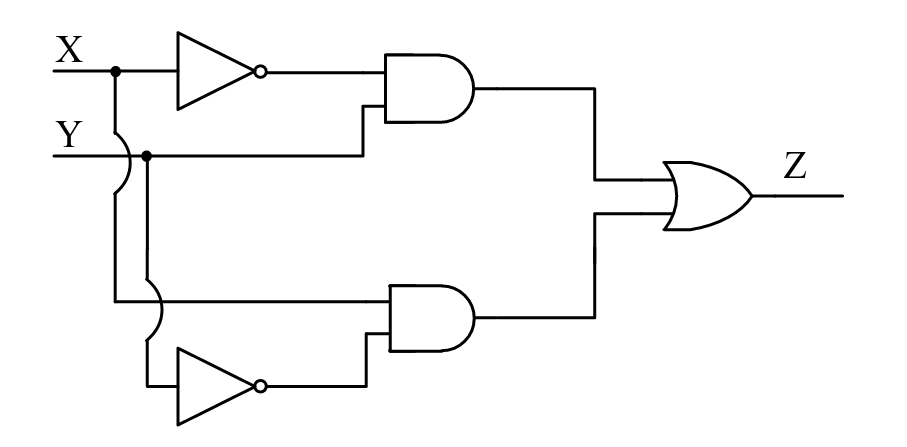
\includegraphics[width=\columnwidth]{figs/2019-gate-ee-36.png}
\caption{}
\label{fig:2019-gate-ee-36}
\end{figure}
\item 
\label{prob:2018-gate-CS-4}		
Let $\oplus$ and $\odot$ denote the Exclusive OR and Exclusive NOR operations, respectively.Which one of the following is NOT CORRECT ?
\ref{prob:2018-gate-CS-4}
\hfill (GATE CS 2018)
\begin{samepage}
\begin{enumerate}[label=(\Alph*)]
    \item $\overline{P\oplus Q}$ = $ P \odot Q $
    \item $\overline{P} \oplus Q$ = $ P \odot Q $
    \item $\overline{P} \oplus \overline{Q}$ = $ P \oplus Q $
    \item $(P \oplus \overline{P}) \oplus Q$ = $(P \odot \overline{P}) \odot \overline{Q}$
\end{enumerate}
\end{samepage}

\item A Boolean digital circuit is composed using two 4-input multiplexers $(M1 and M2)$ and one 2-input multiplexer $(M3)$ as shown in the 
    \figref{fig:Multiplexer}.
	 $X0$–$X7$ are the inputs of the multiplexers $M1$ and $M2$ and could be connected to either $0$ or $1$. The select lines of the multiplexers are connected to Boolean variables $A$, $B$ and $C$ as shown.

\begin{figure}[!ht]
    \centering
        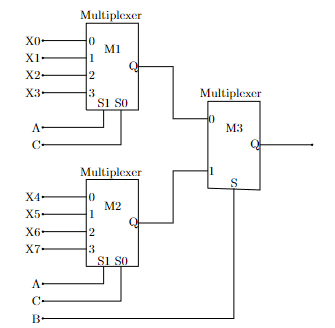
\includegraphics[width=\columnwidth]{figs/Multiplexer.png}
    \caption{Digital Circuit}
    \label{fig:Multiplexer}
\end{figure}

Which one of the following set of values of $(X0, X1, X2, X3, X4, X5, X6, X7)$ will realise the Boolean function 
$\overline{A} + \overline{A}.\overline{C}+A.\overline{B}.C $ ?
\hfill(GATE CS2023,44)
 \begin{enumerate}
     \item (1, 1, 0, 0, 1, 1, 1, 0)
     \item (1, 1, 0, 0, 1, 1, 0, 1)
     \item (1, 1, 0, 1, 1, 1, 0, 0)
     \item (0, 0, 1, 1, 0, 1, 1, 1)
 \end{enumerate}
\item For the given digital circuit
in	\figref{fig:Image},
	 $A = B = 1$. Assume that AND, OR, and NOT gates have propagation delays of $10\mathrm{ns}$,$10\mathrm{ns}$, and $5\mathrm{ns}$ respectively. All lines have zero
propagation delay. Given that $C = 1$ when the circuit is turned on, the frequency of steady-state oscillation of the output $Y$  is  \rule{30pt}{1pt}.
\hfill (GATE IN 2023)
\begin{figure}[!ht]
        \centering  
        
        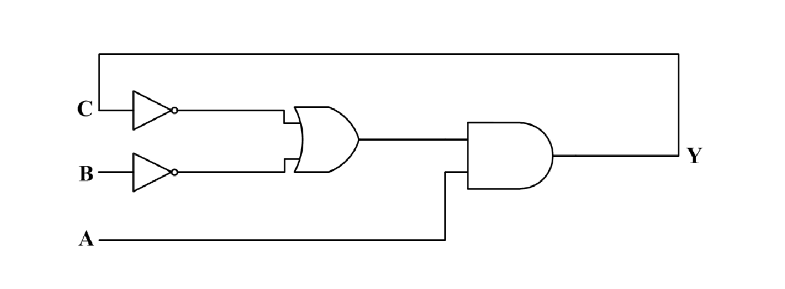
\includegraphics[width=\columnwidth]{figs/gate.png}
        \caption{Image}
	\label{fig:Image}
\end{figure}
    \begin{enumerate}
        \item $20 \mathrm{MHz}$
        \item $15 \mathrm{MHz}$
        \item $40 \mathrm{MHz}$
        \item $50 \mathrm{MHz}$
    \end{enumerate}
\item Select the Boolean function(s) equivalent to $x + yz$, where $x,y$, and $z$ are Boolean variables, and + denotes logical OR  operation.\hfill(GATE EC 2022)
	\begin{enumerate}[label=(\Alph*)]
		\item $x + z + {xy}$
		\item ${(x + y)}{(x + z)}$
		\item $x + {xy} + {yz}$
		\item $x + {xz} + {xy}$
	\end{enumerate}
 \item Which one of the following options is CORRECT for the given circuit 
			in \figref{fig:xxxx}?
	 \hfill(GATE PHYSICS 2023)
		\begin{figure}[!ht]
			\centering
			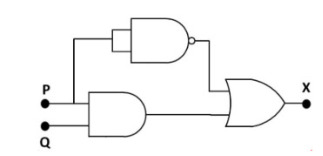
\includegraphics[width=\columnwidth]{figs/Q24.jpg}
			\caption{}
			\label{fig:xxxx}
		\end{figure}

		\begin{enumerate}[label=(\Alph*)]
		\item P = $1$, Q = $1$ ; X = $0$
		\item P = $1$, Q = $0$ ; X = $1$
		\item P = $0$, Q = $1$ ; X = $0$
		\item P = $0$, Q = $0$ ; X = $1$
	\end{enumerate}

\item In the circuit diagram shown below
in \figref{fig:GATE Digram}, the logic gates operate with a supply voltage of $1 V$. NAND and XNOR have $200$ps and $400$ps input-to-output delay, respectively.

At time $t=T.A(t)=0,B(t)=1 and Z(t)=0.$ When the inputs are changed to $A(t)=1,B(t)=0 \text{at} t=2T$, a 1 V pulse is observed at $Z$. the pulse width of the $1 V$ pulse is  ps.


\hfill{(GATE BM 2022)}

\begin{figure}[!ht]
\centering
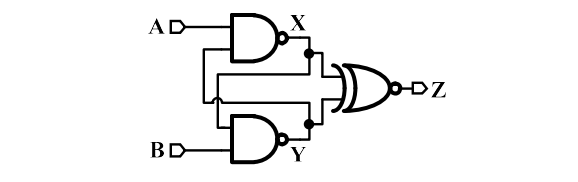
\includegraphics[width=\columnwidth]{figs/bm2022.png}
\caption{}
\label{fig:GATE Digram}
\end{figure}

\begin{enumerate}
\item $100$
\item $200$
\item $400$
\item $600$
\end {enumerate}

\item 
Consider a Boolean gate (D) where the output (Y) is related to the inputs (A) and (B) as, $Y = A + B$, where + denotes logical OR operation. The Boolean inputs '0' and '1' are also available separately. Using instances of only D gates and inputs '0' and '1', (select the correct option(s)).\hfill{(GATE EC 2022)}

\begin{enumerate}
\item  NAND logic can be implemented
\item  OR logic cannot be implemented
\item  NOR logic can be implemented
\item  AND logic cannot be implemented.
\end{enumerate}

\item Let $R1$ and $R2$ be two $4$-bit registers that store numbers in $2$’s complement form.
For the operation $R1+R2$, which one of the following values of $R1$ and $R2$ gives an
arithmetic overflow?
\hfill{(GATE CS 2022)}

    \begin{enumerate}
        \item $R1 = 1011$ and $R2 = 1110$
        \item $R1 = 1100$ and $R2 = 1010$
        \item $R1 = 0011$ and $R2 = 0100$
        \item $R1 = 1001$ and $R2 = 1111$
    \end{enumerate}


\item The maximmunm clock frequeccy in MHz of a $4$-stage ripple counter, utilize flip-flops, with each flip-flop having a propagation delay of $20$ ns, is $\rule{2cm}{0.15mm}$.\\
(\textit{round off to one decimal place})
\hfill{(GATE EE 20222)}

\item The logic block shown 
in
\figref{fig:GATE IN 2021}
	has an output $F$ given by \rule{2cm}{0.15mm}
\hfill (GATE IN 2021)
\begin{figure}[!ht]
\centering
\includegraphics[width=\columnwidth]{figs/gatemage.jpg}
	\caption{}
\label{fig:GATE IN 2021}
\end{figure}
\begin{enumerate}
	\item$A+B$
	\item$A.\bar{B}$
	\item$A+\bar{B}$
	\item$\bar{B}$
\end{enumerate}

\item Consider the following Boolean expression 
\begin{align*} F = (X+Y+Z)(\bar{X}+Y)(\bar{Y}+Z) \end{align*}
       
Which of the following Boolean expressions is/are equivalent to $\overline{F}$ (complement of 
 F)?
 
\hfill{(Gate CS 2021,42)}
\begin{enumerate}                                     
\item $(\bar{X}+\bar{Y}+\bar{Z})(X+\bar{Y})(Y+\bar{Z})$
\item $X\bar{Y}+\bar{Z}$
\item $(X+\bar{Z})(\bar{Y}+\bar{Z})$
\item $X\bar{Y}+Y\bar{Z}+\bar{X}\bar{Y}\bar{Z}$ 
\end{enumerate}

    \item The propagation delays of the XOR gate, AND gate and multiplexer \brak{MUX} in the circut shown in  
\figref{fig:block_diagram}
	    are $4 ns$, $2 ns$ and $1 ns$, respectively.
    If all the inputs $P, Q, R, S$ and T are applied simultaneously and held constant, the maximum propagation delay of the circuit is
\hfill(GATE-EC2021,31)  

\begin{figure}[!ht]
	\resizebox{\columnwidth}{!}{
\begin{circuitikz}
\draw (7,1)coordinate (E) -- (8,1)coordinate (F) -- (8,-1)coordinate (G) -- (7,-1)coordinate (H) -- (7,1)coordinate (E);
\draw (11,2)coordinate (I) -- (13,2)coordinate (J) -- (13,-1)coordinate (K) -- (11,-1)coordinate (L) -- (11,2)coordinate (I);
 \draw ($(J)!0.5!(K)$)--++(0:2)node[right]{$Y$};
 \draw ($(L)!0.5!(K)$)node[anchor=south]{$S0$}--++(90:-2)--++(1:-10)node[left]{$T$};
 \draw ($(H)!0.5!(G)$)node[anchor=south]{$S0$}--++(90:-2)--++(1:0)node[left]{};
\draw (4,2) node[and port] (myand1) {};
\draw (myand1.in 1) node (A1)     [anchor=east,xshift=-1cm]           {$P$}
(myand1.in 1) -- (A1);
\draw(4,-2) node[and port] (myand2) {}
(myand2.in 2) node (B2)     [anchor=east,xshift=-1cm]           {$S$};
\draw(myand2.in 2) -- (B2);
\draw (10,0) node[and port] (myand3) {};
\draw (4,0) node[xor port] (myxor) {};
\draw (myand1.in 2) node (B1)     [anchor=east,xshift=-1cm,yshift=-.7cm]  {$Q$};
\draw (B1) -- ++(1.25cm,0);
\draw (myxor.in 1) node (B1)     [anchor=east,xshift=-1cm,yshift=-1.3cm]  {$R$};
\draw (B1) -- ++(1.25cm,0);

\draw (myand1.in 2) |- (myxor.in 1);
\draw (myand2.in 1) |- (myxor.in 2);

\draw (myxor.out) |- ($(E)!0.2!(H)$)--++(0:0)node[right]{$0$};
\draw(myand1.out) |- ($(I)!0.2!(L)$)--++ (0:0)node[right]{$0$};
\draw (myand1.out) -| (myand3.in 1);
\draw(myand3.out) -| ($(I)!0.7!(L)$)--++(0:0)node[right]{$1$};
\draw ($(F)!0.6!(G)$)--++(0:0)node[right]{} -| (myand3.in 2) ;
\draw (myand2.out) |- ($(E)!0.7!(H)$)--++(0:0)node[right]{$1$};

\end{circuitikz}
~


	}
\caption{circuit daigram} 
\label{fig:block_diagram}
\end{figure}
\begin{enumerate}

    \item $3 ns$
    \item $5 ns$
    \item $6 ns$
    \item $7 ns$
\end{enumerate}
\item  The following combination of logic gates
in
		      \figref{fig:GATE PH 2021}
	represent the operation
 \hfill(GATE PH 2021)
	      \begin{figure}[!ht]
		      \centering
		      \resizebox{\columnwidth}{!}{%
		                   \begin{circuitikz}
              
                  \draw (2,5) node[not port,scale=2] (not) {};
                  \draw (not.in) -- ++(-0.5,0);
                  \draw (not.out) -- ++(0.5,0) ;
                  
                
                
                \draw (7.5,3) node[or port,scale=2] (orgate) {};
                  \draw (orgate.in 1) -- ++(-0.5,0) ;
                  \draw (orgate.in 2) -- ++(-0.5,0);
                  \draw (orgate.out) -- ++(0.5,0) ;
                
                 \draw (2,1) node[not port,scale=2] (notgate) {};
                  \draw (notgate.in) -- ++(-0.5,0) ;
                  \draw (notgate.out) -- ++(0.5,0) ;
                
                \draw (notgate.out) -- ([xshift=0.5cm]notgate.out) |-(orgate.in 2);
                  
                \draw (not.out) -- ([xshift=0.5cm]not.out) |-(orgate.in 1);
                  
            \end{circuitikz}

		      }
	              \caption{combination circuit}
		      \label{fig:GATE PH 2021}
	      \end{figure}

	\begin{enumerate}
       \item OR
       \item NAND
       \item AND
       \item NOR
   \end{enumerate}
\item Consider the boolean Function $z\brak{a,b,c}$ from below 
			\figref{fig:203}.
		\begin{figure}[!ht]
			\centering
			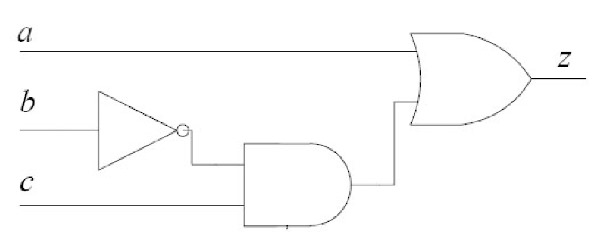
\includegraphics[width=\columnwidth]{figs/203.png}
			\caption{circuit diagram}
			\label{fig:203}
		\end{figure}
		
	\hfill{(Gate CS-2020)}
	
		Which of the following minterm lists represent the circuit given above?
	\begin{enumerate}
		\item $z=\Sigma\brak{0,1,3,7}$
		\item $z=\Sigma\brak{1,4,5,6,7}$
		\item $z=\Sigma\brak{2,4,5,6,7}$
		\item $z=\Sigma\brak{2,3,5}$
	\end{enumerate}	   
\item In the latch circuit shown
in
\figref{figure_1}, the NAND gates have non-zero but unequal propagation delays. The present input condition is: $P=Q=\lq 0\rq$. If the input condition is changed simultaneously to $P=Q=\lq 1\rq$,the outputs $X$ and $Y$ are 
\begin{figure}[!ht]
\centering
\resizebox{\columnwidth}{!}{%
\begin{circuitikz}
    \draw (0,0) node[nand port] (nand1) {};
    \draw (0,-2) node[nand port] (nand2) {};
    \draw (nand1.in 1) -- ++(-0.5,0) node[left] {$P$};
    \draw (nand1.in 2) -- ++(-0.2,0) coordinate (in1);
    \draw (nand1.out) -- ++(0.1,0) coordinate (out1); 
    \draw (nand2.in 1) -- ++(-0.2,0) coordinate (in2);
    \draw (nand2.in 2) -- ++(-0.5,0) node[left] {$Q$};
    \draw (nand2.out) -- ++(0.1,0) coordinate (out2);
    \draw (out2)-- ++(0,0.5)-- ++(-2,1) |- (in1);
    \draw (out1)-- ++(0,-0.5)-- ++(-2,-1) |- (in2);
    \draw (out1) -- ++(1,0) node[above right] {X};
    \draw (out2) -- ++(1,0) node[above right] {Y};
\end{circuitikz}

	}
	\caption{}
\label{figure_1}
\end{figure}
\begin{enumerate}
\item $X=\lq 1\rq,Y=\lq 1 \rq$
\item either $X=\lq 1\rq,Y=\lq 0\rq$ or $X=\lq 0\rq,Y=\lq 1\rq$
\item either $X=\lq 1\rq,Y=\lq 1\rq$ or $X=\lq 0\rq,Y=\lq 0\rq$
\item $X=\lq 0\rq,Y=\lq 0 \rq$
\end{enumerate}
\hfill(GATE EC 2017)

\item Consider three $4$-variable functions $f_1, f_2, $and $f_3,$ which are expressed in sum-of-minterms as \newline \quad $f_1 = \sum\brak{0,2,5,8,14}$, \quad $f_2=\sum\brak{2,3,6,8,14,15}$, \quad $f_3 = \sum\brak{2,7,11,14}$ \newline For the following circuit 
	in 
	\figref{fig:GATE-CS2019,30}
	with one AND gate and one XOR gate, the output function $f$ can be expressed as:
	\hfill(GATE-CS2019,30)
	\begin{figure}[!ht]
		 \centering
		 \resizebox{\columnwidth}{!}{%
			\begin{circuitikz}
    % Draw AND gate
    \draw (0,0) node[and port] (and) {AND};
    
    % Draw XOR gate
    \draw (4,-0.2) node[xor port] (xor) {XOR};
    
    % Connect AND output to XOR input
    \draw (and.out) -- (xor.in 1);
    
    % Draw input wires
    \draw (and.in 1) -- ++(-1,0) node[left] {$f_1$};
    \draw (and.in 2) -- ++(-1,0) node[left] {$f_2$};
    \draw (xor.in 2)--++(-90:2) --++(-5,0) node[left] {$f_3$};    % Draw XOR output
    \draw (xor.out) -- ++(1,0) node[right] {$f$};
\end{circuitikz}


			}
                 \caption{Circuit Daigram}
	\label{fig:GATE-CS2019,30}
	\end{figure}
		\begin{enumerate}
		\item $\sum\brak{7,8,11}$
		\item $\sum\brak{2,7,8,11,14}$
		\item $\sum\brak{2,14}$
		\item $\sum\brak{0,2,3,5,6,7,8,11,14,15}$
		\end{enumerate}

\item In the circuit shown
	in \figref{fig:GATE-EC2019,14},
	what are the values of $F$for $EN=0$ and $EN=1$,  respectively?
 \hfill(GATE-EC2019,14)  

\begin{figure}
    \centering
    \resizebox{\columnwidth}{!}{%
    \begin{circuitikz}

\draw (0.5,1) node[nand port] (nand) {};
\draw (nand.in 1) -- ++(-1.7,0) node[left] {};
\draw (nand.in 2) -- ++(-2.2,0) node[left] {EN};
\draw (nand.out) -- ++(0.5,0) node[midway, above] {};
\draw (0.5,-3) node[nor port] (nor) {};
\draw (nor.in 1) node[left] {};
\draw (nor.in 2) --++(-2.2,0) node[left] {D};
\draw (nor.out) -- ++(0.5,0) node[midway, above] {};
\draw (-1.6,-1) node[rotate=270,not port] (not) {};
\draw (not.in) |-(nand.in 2);
\draw  (nor.in 1) -| (not.out);
\draw (2,1) node[pmos] (pmos) {};
\draw (2,-3) node[nmos] (nmos) {};
\draw (nand.out) -- (pmos.gate);
\draw (nor.out) -- (nmos.gate);
\draw(nand.in 1) -- ++(-1.7,0) |- (nor.in 2) -- ++(-1,0);
\draw (pmos.drain) -- (nmos.drain);
\draw (pmos.drain)--++(90:-1)--++(2:1)node[left, yshift=0.2cm]{$F$};
\draw (nmos.source) -- (nmos.source |- 0,-4) node[ground] {};
\draw(2,1.7) node[rground,yscale=-1] {};
\draw(2,2.3) node(right) {$V_{DD}$};

\end{circuitikz}


	}
    \caption{Circuit Diagram}
	\label{fig:GATE-EC2019,14} 
\end{figure}
\begin{enumerate}
    \item $0$ and $D$
    \item $Hi-Z$ and $D$
    \item $0$ and $1$
    \item $Hi-Z$ and $\overline{D}$
\end{enumerate}
\item In the circuit shown
	   in \figref{fig:GATE-EC2019,15},
	$A$ and $B$ are the inputs and $F$ is the output. What is the functionality of the circuit?
           \hfill(GATE-EC2019,15)
           
\begin{figure}[!ht]
\centering
\resizebox{\columnwidth}{!}{%

\begin{circuitikz}
    % Draw PMOS transistors
     \draw (2,1) node [pmos] (pmos1) {};
    \draw (2,0) node [pmos,rotate=180] (pmos2) {};
    \draw (0,-2) node [nmos,rotate=180] (nmos1) {};
    \draw (4,-2) node [nmos] (nmos2) {};
    
    % connections
     \draw(pmos1.gate)  -- (nmos1.gate);
      \draw(pmos2.gate) -- (nmos2.gate);
     \draw (pmos1.drain) -- (pmos2.drain);
    \draw (nmos1.source) -- (nmos2.drain);
    \draw (nmos1.gate) --(nmos2.source);
    \draw (nmos2.gate) -- (nmos1.drain);
    \draw (pmos2.source) -- (2,-1.22);
    \draw (nmos2.drain) -- (4,-1.22) node[circ]{};
    \draw (nmos2.drain)node[anchor=east,xshift=0.45cm,yshift=-0cm] 
    {$F$};
    %%B
    \draw (nmos2.source) node[circ]{};
    \draw (nmos2.source)node[anchor=east,xshift=0.48cm,yshift=-0cm] {$B$};
    %%A
    \draw (nmos1.drain)node[circ]{};
     \draw (nmos1.drain)node[anchor=east,xshift=0cm,yshift=-0cm] {$A$};
     %%vdd
    \draw (2,1.75) node[rground,yscale=-1] {};
    \draw (2.5,1.8) node(right) {$V_{DD}$};
\end{circuitikz}


	}
\caption{Circuit Diagram}
	   \label{fig:GATE-EC2019,15}
\end{figure}
\begin{enumerate}
\item Latch
\item XNOR
\item SRAM Cell
\item XOR
\end{enumerate}

\item In the circuit shown below in 
	    \figref{fig:GATE-IN2019,34},
	 assume that the comparators are ideal and all components have zero propagation delay. In one period of the input signal $Vin=6\sin\brak{\omega t}$, the fraction of the time for which the output OUT is in logic HIGH is 
		                 \hfill(GATE-IN2019,34)
\begin{figure}[!ht]
\centering
\resizebox{\columnwidth}{!}{%
    \begin{circuitikz}

\draw (0,0) node[op amp] (opamp1) {};
\draw (opamp1.-)  node[left]{};
\draw (opamp1.+) node[left]{};
\draw (opamp1.out) node[right]{} ;
\draw (0,5) node[op amp] (opamp2) {};
\draw (opamp2.-)  node[left]{};
\draw (opamp2.+)  node[left]{};
\draw (opamp2.out) node[right]{};
\draw (3.5,5) node[not port] (notgate1) {};
\draw (notgate1.in) node[left] {};
\draw (notgate1.out) node[right] {};
\draw (3.5,2) node[not port] (notgate2) {};
\draw (notgate2.in) node[left] {};
\draw (notgate2.out) node[right] {};
\draw (6.5,3.5) node[and port] (andgate1) {};
\draw (andgate1.in 1) node[left] {};
\draw (andgate1.in 2)  node[left] {};
\draw (andgate1.out) node[right] {};
\draw (6.5,0.5) node[and port] (andgate2) {};
\draw (andgate2.in 1) node[left] {};
\draw (andgate2.in 2)  node[left] {};
\draw (andgate2.out) node[right] {};
\draw (8,2) node[or port] (orgate) {};
\draw (orgate.in 1) node[left] {};
\draw (orgate.in 2)  node[left] {};
\draw (orgate.out) node[right] {$out$};
\draw (andgate1.out) -| (orgate.in 1);
\draw (andgate2.out) -| (orgate.in 2);
\draw (notgate1.out) -| (andgate1.in 1);
\draw (notgate2.out) -| (andgate1.in 2);
\draw (opamp2.out) -|(notgate1.in);
\draw (opamp1.out) -| (andgate2.in 2);
\draw(opamp2.out)--++(90:0)|-(andgate2.in 1);
\draw(notgate2.in)--++(50:0)|-(opamp1.out);
\draw(opamp1.-)--++(90:0)-|(-3,2)|-(opamp2.-);
\draw(opamp2.+)--++(0,-1) node[rground,rotate=180,yscale=-1]{};
\draw (-1.2,2.8)node(right) {$3V$};
\draw(opamp1.+)--++(0,-1) node[ground,rotate=180,yscale=-1]{};
\draw (-5,5.5) to[sV] (-5,0)node[ground,rotate=180,yscale=-1]{};
\draw (-5,5.5) -- (opamp2.-);
\draw (-6,3)node(right) {$6 \sin{\omega t}$};
\draw (0,5.5) -- (0,6.2)node(right) {};
\draw (0,6.5) node(right) {$HIGH$};
\draw (0,4.5) -- (0,3.8)node(right) {};
\draw(0,3.5) node(right) {LOW};
\draw (0,0.5) -- (0,1.2)node(right) {};
\draw (0,1.5) node(right) {$HIGH$};
\draw (0,-0.5) -- (0,-1.2)node(right) {};
\draw (0,-1.5) node(right) {$LOW$};

\end{circuitikz}


	}
	    \caption{Circuit Daigram}
	    \label{fig:GATE-IN2019,34}
     \end{figure}
\begin{enumerate}
	\item $\dfrac{1}{12}$
	\item $\dfrac{1}{2}$
	\item $\dfrac{2}{3}$
	\item $\dfrac{5}{6}$
\end{enumerate}


\item 
	\figref{fig:GATE-IN2019,22}
	shows the $ith$ full-adder block of a binary adder circuit. $C_i$ is the input carry and $C_{i+1}$is the output carry of the circuit. Assume that each logic gate has a delay of $2$ nanosecond, with no additional time delay due to the interconnecting wires. If the inputs $A_i$ , $B_i$; are available and stable throughout the carry propagation, the maximum time taken for an input $C_i$, to produce a steady-state output $C_{i+1}$ is $\underline{\hspace{18pt}}$ nanosecond.
	               \hfill(GATE-IN2019,22)
\begin{figure}[!ht] 
    \centering
    \resizebox{\columnwidth}{!}{%
	\begin{circuitikz}
    \draw (0,0) node[xor port] (xor1) {};
    \draw (xor1.out)  node[right] {};
    \draw (xor1.in 1) -- ++(-0.52,0) node[left] {$B_i$};
    \draw (xor1.in 2) -- ++(-1,0) node[left] {$A_i$};
    
    \draw (5,0) node[xor port] (xor2) {};
    \draw (xor2.out) node[right] {$S_i$};
    \draw (xor2.in 1)  node[left] {};
    \draw (xor2.in 2) |- (2,-2.29) node[below] {$C_i$};
    % First AND gate
    \draw (6,-2) node[and port] (and1) {};
    \draw (and1.out) node[right] {};
    \draw (and1.in 1) node[left] {};
    \draw (and1.in 2)  node[left] {};
    
    % Second AND gate
    \draw (0,-2) node[and port] (and2) {};
    \draw (and2.out)  node[right] {};
    \draw (and2.in 1)  node[left] {};
    \draw (and2.in 2)  node[left] {};
    \draw (9,-3) node[or port] (or) {};
    \draw (or.out) -- ++(0,0) node[right] {$C_{i+1}$};
    \draw (or.in 1) -- ++(-0.5,0) node[left] {};
    \draw (or.in 2) -- ++(-0.5,0) node[left] {};
   \draw (xor1.in 1) -- ++(-0.5,0) |- (and2.in 1);
   \draw (xor1.in 2) -- ++(-1,0) |- (and2.in 2);
    \draw(xor1.out)  --++(1,0)   |- (xor2.in 1);
    \draw(xor2.in 1)--++(-2,0)   |-(and1.in 1);
   % \draw(xor2.in 2)--++(-3,0)   |-(and1.in 2);
    \draw (and1.out)--++(0,-0.7) |-(or.in 1);
     \draw (and2.out)--++(0,-0.7) |-(or.in 2);
     \draw(xor2.in 2) |-(and1.in 2);
    \end{circuitikz}



	}
	\caption{Full Adder}
	\label{fig:GATE-IN2019,22}
\end{figure}
\item The Boolean operation performed by the following  circuit 
in
\figref{fig:figure13}
	at the output $O$ is \underline{\hspace{2cm}}
    $\hfill\brak{GATE \enspace IN2020-12}$

\begin{figure}[!ht]
	\centering
	\resizebox{\columnwidth}{!}{%
    \begin{circuitikz}[circuit logic IEC]
        
        \node[and gate, inputs={nnnn}, and gate IEC symbol={}, text height=6cm, text width=3cm] (A) at  (0,0){}; 
        \draw (-2.55,0.62) -- ++(-3.2,0);
        \draw (-2.55,-0.62) -- ++(-3.2,0); 
        \draw (-2.55,-1.85) -- ++(-5.5,0); 
        \draw (-5.7,-0.65) -- ++(0,2.5); 
        \draw (-8,-1.9) -- ++(0,3.72); 
        \node at (0.6,2.5) [anchor=north east] {4:1};
        \node at (0.8,2) [anchor=north east] {Mux};
        \node[anchor=east] at ([xshift=0.6cm]A.input 1) {$I_0$};
        \node[anchor=east] at ([xshift=0.6cm]A.input 2) {$I_1$};
        \node[anchor=east] at ([xshift=0.6cm]A.input 3) {$I_2$};
        \node[anchor=east] at ([xshift=0.6cm]A.input 4) {$I_3$};
       \draw ([xshift=-0.6cm]A.output) node[right] {$O$};

        \draw (A.output) -- ++(0.2,0); 
        \foreach \i in {1,...,4}
            \draw (A.input \i) -- ++(-1,0);
        \draw (A.output) -- ++(1,0);
        \node[not port] (not_gate) at (-4.5,1.85) {};
        \draw (not_gate.out) -- ++(1.2,0);
        \draw (not_gate.in) -- ++(-1,0);
        \node[not port] (not_gate) at (-6.9,1.85) {};
        \draw (not_gate.in) -- ++(-1.9,0);
        \draw (-9.49,-1.67) -- ++(0,3.5); 
        \draw (-9.49,-1.67) node[ground] {};
        \path (A.south) -- ++(0,-0.5) coordinate (bottom_center);
    
        \draw (A.south) ++(-0.5,0) -- ++(0,-0.5) node[below] {$s_1$};
        \draw (A.south) ++(0.5,0) -- ++(0,-0.5) node[below] {$s_0$};
      
        \node[below] at ($(A.south) + (-0.7,-0.9)$) {MSB};
       
        \node[below] at ($(A.south) + (0.7,-0.9)$) {LSB};
    \end{circuitikz}

	}
\caption{Circuit Diagram}
\label{fig:figure13}
\end{figure}

\begin{enumerate}

            \item  $O=S_1\oplus S_0$ 
            
            \item  $O=S_1\bullet\overline{\rm S_0}$
            
            \item  $O=S_1 + S_0$
            
            \item $O=S_0\bullet\overline{\rm S _1}$
 \end{enumerate}
\item  The chip select logic for a certain DRAM chip in a memory system design is shown below
	in
\figref{fig:figure14}.
	Assume that the memory system has 16 address lines denoted by ${A_{15}}$ to ${A_0}$. What is the range of addresses (in hexadecimal) of the memory system that can get enabled by the chip select (CS) signal?
\hfill{\brak{GATE \enspace CS2019-2}}

\begin{figure}[!ht]
\begin{center}
\begin{circuitikz}
\draw ((5,5) node[ieeestd and port,number inputs=5,minimum height=5cm, minimum width=5cm, anchor=in 1] (B) {} (B.in 1) node[anchor=east] {$A_{15}$}(B.in 2) node[anchor=east] {$A_{14}$}(B.in 3) node[anchor=east] {$A_{13}$}(B.in 4) node[anchor=east] {$A_{12}$}(B.in 5) node[anchor=east] {$A_{11}$}(B.out) node[anchor=west] {$CS$};
\node at (B.bin 3) [ocirc, left]{} ;
\node at (B.bin 4) [ocirc, left]{};
\end{circuitikz}  
\end{center}
\caption{Logic Diagram}
\label{fig:figure14}
\end{figure}

\begin{enumerate}
\item ${C800}$ to ${CFFF}$
\item ${CA00}$ to ${CAFF}$
\item ${CA00}$ to ${C8FF}$
\item ${DA00}$ to ${DFFF}$
\end{enumerate}  


\item A $6{\frac{1}{2}}$ digit time counter is set in the time period mode of operation and range is set as 'ns'. For an input signalthe time-counter displays $1000000$. with the same input signal,The time countr is changed to 'frequency' mode of operation and the range is set as 'HZ'.The display will be show the number$\underline{\hspace{2cm}}$.
\hfill{\brak{GATE \enspace IN2020-43}}


\item  A $2\times2$ ROM array is built with the help of diodes as shown in the circuit below
	in \figref{fig:2rom}. Here $W0$ and $W1$ are signals that select the word lines and $B0$ and $B1$ are signals that are output of the sense amps based on the stored data corresponding to the bit lines during the read operation.
%
\begin{figure}[!ht]
        \centering
	\resizebox{\columnwidth}{!}{%
        \begin{circuitikz} 
\draw (2,0) node[nmos] {} (3,0)
(4,0) node[nmos] {} (5,0)
(4,-0.375) node[ground] {}
(2,-0.375) node[ground] {}
;
\ctikzset{diodes/scale=0.6} 
\draw  (1,3) to[empty diode] (2,2.25)
(3,1.5) to[empty diode ] (4,0.75)
;
\ctikzset{diodes/scale=1} 

\draw [very thick](1.75,3.75) -- (2,4.25) -- (2.25,3.75) -- cycle
(3.75,3.75) -- (4,4.25) -- (4.25,3.75) -- cycle
(0,0) -- (2,0) -- (5,0)
(0,1.5) node[anchor=east] {W1}--  (5,1.5)
(0,0) -- (0,0.625)
(-0.25,1.2) node[anchor=north] {VDD}
(2,4.25) -- (2,4.6) node[anchor=south] {B0}
(4,4.25) -- (4,4.6) node[anchor=south] {B1}
(-0.15,0.55) -- (0,0.625) --(0.15,0.7)
(0,3) node[anchor=east] {W0}  -- (5,3)
(2,0.25) --  (2,3.75)
(4,0.25) -- (4,3.75)
(8.125,1.75) -- (8,1.75) -- (8,3) --(8.125,3)
(9.625,1.75) -- (9.75,1.75) -- (9.75,3) --(9.625,3);
\node (mynode) at (3,4) {\scalebox{0.5}{Sense amps}};
 \filldraw[fill=black, draw=black] (1,3) circle [radius=0.1];
 \filldraw[fill=black, draw=black] (2,2.25) circle [radius=0.1];
 \filldraw[fill=black, draw=black] (3,1.5) circle [radius=0.1];
 \filldraw[fill=black, draw=black] (4,0.75) circle [radius=0.1];
 %matrix code
\node at (8.5,3.5) {$B_{0}$};
\node at (9.25,3.5) {$B_{1}$} ;
\node at (7.4,2.75) {$W_{0}$};
\node at (8.5,2.75) {$D_{00}$};
\node at (9.25,2.75) {$D_{01}$};
\node at (7.4,2) {$W_{1}$};
\node at (8.5,2) {$D_{10}$};
\node at (9.25,2) {$D_{11}$};
\node at (8.7,1) {Bits stored in the ROM Array};


\end{circuitikz}

	}
        \caption{ $2\times 2$ ROM array}
	\label{fig:2rom}
\end{figure}
%
		During the read operation, the selected word line goes high and the other word line is in a high impedance state. As per the implementation shown in the circuit diagram above, what are the bits corresponding to $D_{ij}\brak{\text{where $i=0$ or $1$ and $j=0$ or $1$}}$ stored in the ROM?
	\hfill(GATE EC2018,32)
\begin{enumerate}
    \item \myvec{1 & 0\\0 & 1}
    \item \myvec{0 & 1\\1 & 0}
    \item \myvec{1 & 0\\1 & 0}    
    \item \myvec{1 & 1\\0 & 0}
\end{enumerate}

\item The two inputs A and B are connected to to an R-S latch via two AND gates as shown in  
       \figref{fig:GATE IN2017,43}.
If $A=1$ and $B=0$, the output $Q\bar{Q}$ is
    \begin{figure}[!ht]
        \centering
	\resizebox{\columnwidth}{!}{%
        \begin{circuitikz}
    %input nodes
  \draw (0,0) node[circ] (A) {};
  \draw (0,-0.6) node[circ] (Qb) {};
  \draw (0,-1.6) node[circ] (Q) {};
  \draw (0,-2.2) node[circ] (B) {};
      \draw (A) ++(180:0.5) node {A};
      \draw (Qb) ++(240:0.5) node {$\bar{Q}$};
      \draw (Q) ++(210:0.5) node {Q};
      \draw (B) ++(200:0.5) node {B};    
  %and Gate
  \draw (2,-0.3) node[and port] (anda){};
  \draw (A) -- (anda.in 1);
  \draw (Qb) -- (anda.in 2);
  \draw (2,-1.9) node[and port] (andb){};
  \draw (Q) -- (andb.in 1);
  \draw (B) -- (andb.in 2);
  
  %latch
  \draw (4,-1.1) node[flipflop SR] (SR) {\tiny R-S Latch};
  \draw (anda.out) |- (SR.pin 1);
  \draw (andb.out) |- (SR.pin 3);
  
  \draw (Qb) to ++(-1,0) to[crossing] ++(0,-2) to ++(7,0) to[short,-*] ++(0,0.65) |- (SR.pin 4);
  \draw (0,-1.6) to ++(-1.5,0) to ++(0,+2) to ++(7.5,0) to[short,-*] ++(0,-0.65) |- (SR.pin 6);
  
   \end{circuitikz}
	    }
	    \caption{}
       \label{fig:GATE IN2017,43}
       \end{figure}
       \hfill(GATE IN2017,43)
    \begin{enumerate}
   		\item $00$ 
   		\item $10$ 
   		\item $01$ 
   		\item $11$ 
   
   \end{enumerate}
\item $A$ and $B$ are logical inputs and $X$ is the logical output shown in 
\figref{fig:gate_in_2017_30}.
	The output $X$ is related to $A$ and $B$ by \hfill{(GATE IN 2017)}
\begin{figure}[!ht]
\centering
\resizebox{\columnwidth}{!}{%
\begin{circuitikz}
\tikzstyle{every node}=[font=\normalsize]
\draw (7.75,11.5) node[ieeestd not port, anchor=in](port){} (port.out) to[short] (10.5,11.5);
\draw (port.in) to[short] (6.5,11.5);
\draw (7.75,9.5) node[ieeestd not port, anchor=in](port){} (port.out) to[short] (10.25,9.5);
\draw (port.in) to[short] (6.75,9.5);
\draw (11.75,10.75) to[short] (12,10.75);
\draw (11.75,10.25) to[short] (12,10.25);
\draw (12,10.75) node[ieeestd and port, anchor=in 1, scale=0.89](port){} (port.out) to[short] (14,10.5);
\draw (8,7.5) to[short] (8.25,7.5);
\draw (8,7) to[short] (8.25,7);
\draw (8.25,7.5) node[ieeestd and port, anchor=in 1, scale=0.89](port){} (port.out) to[short] (10,7.25);
\draw (14,10.5) to[short] (14,10.5);
\draw (14,10) to[short] (14,10);
\draw (14,10.5) node[ieeestd or port, anchor=in 1, scale=0.89](port){} (port.out) to[short] (15.75,10.25);
\draw[] (6.75,9.5) to[short] (4.25,9.5);
\draw [](5.75,9.5) to[short] (5.75,7);
\draw[] (8,7) to[short] (5.75,7);
\draw[] (8,7.5) to[short] (6.5,7.5);
\draw [](6.5,8) to[short] (6.5,7.5);
\draw[] (11.75,10.75) to[short] (10.5,10.75);
\draw[] (11.75,10.25) to[short] (10.5,10.25);
\draw [](10.5,10.25) to[short] (10.5,9.5);
\draw[] (10.5,9.5) to[short] (10.25,9.5);
\draw [](14,10) to[short] (14,7.5);
\draw [](10,7.25) to[short] (14,7.25);
\draw [](14,7.25) to[short] (14,7.75);
\draw [](10.5,11.5) to[short] (10.5,10.75);
\draw[] (6.5,11.5) to[short] (4.25,11.5);
\draw [](6.5,8) to[short] (6.5,9.25);
\draw [](6.5,11.5) to[short] (6.5,9.75);
\draw [](6.5,10) to[short] (6.5,9.25);
\draw [](4.25,9.5) to[short, -o] (3.75,9.5);
\draw [](4.25,11.5) to[short, -o] (3.75,11.5);
\node [font=\normalsize] at (3.5,11.5) {A};
\draw [](15.75,10.25) to[short, -o] (16.25,10.25);
\node [font=\normalsize] at (3.5,9.5) {B};
\node [font=\normalsize] at (16.5,10.25) {X};
\draw (5.75,9.5) to[short, -*] (5.75,9.5);
\draw (6.5,11.5) to[short, -*] (6.5,11.5);
\end{circuitikz}

	}
\caption{Logic Gate Structure}
\label{fig:gate_in_2017_30}
\end{figure}
\begin{enumerate}[label=\Alph*.]
\item $X = \overline{A}B + \overline{B}A$
\item $X = AB + \overline{B}A$
\item $X = AB + (\overline{B})(\overline{A})$
\item $X = (\overline{A})(\overline{B}) + \overline{B}A$
\end{enumerate}


\item The functionality implemented by the circuit below 
in
\figref{fig:gate_ec_2016_43}
	is \hfill{(GATE 2016 EC)}

\begin{figure}[!ht]
\centering
\resizebox{\columnwidth}{!}{%

\begin{circuitikz}[scale=1.1]
\tikzstyle{every node}=[font=\large]
\draw  (5,10.75) rectangle (7.75,7);
\draw [](4.75,16) to[short] (11.75,16);
\draw [](4.75,14.75) to[short] (11.75,14.75);
\draw [](4.75,13.25) to[short] (11.75,13.25);
\draw [](4.75,17.5) to[short] (11.75,17.5);
\draw (11.5,17.5) node[ieeestd buffer port, anchor=in](port){} (port.out) to[short] (13.25,17.5);
\draw (port.in) to[short] (11.25,17.5);
\draw (11.5,16) node[ieeestd buffer port, anchor=in](port){} (port.out) to[short] (13.5,16);
\draw (port.in) to[short] (11,16);
\draw (11.5,14.75) node[ieeestd buffer port, anchor=in](port){} (port.out) to[short] (13,14.75);
\draw (port.in) to[short] (11.5,14.75);
\draw (11.5,13.25) node[ieeestd buffer port, anchor=in](port){} (port.out) to[short] (13.25,13.25);
\draw (port.in) to[short] (11.25,13.25);
\draw [](12.25,17.25) to[short] (12.25,16.75);
\draw[] (12.25,16.75) to[short] (9.25,16.75);
\draw [](9.25,16.75) to[short] (9.25,10.25);
\draw[] (9.25,10.25) to[short] (7.75,10.25);
\draw [](12.25,15.75) to[short] (12.25,15.5);
\draw[] (12.25,15.5) to[short] (10,15.5);
\draw [](10,15.5) to[short] (10,9.75);
\draw[] (10,9.75) to[short] (7.75,9.75);
\draw [](12.25,14.5) to[short] (12.25,14);
\draw[] (12.25,14) to[short] (10.75,14);
\draw [](10.75,14) to[short] (10.75,9.25);
\draw [](10.75,9.25) to[short] (10.75,8.75);
\draw[] (10.75,8.75) to[short] (7.75,8.75);
\draw [](12.25,13) to[short] (12.25,7.75);
\draw[] (12.25,7.75) to[short] (7.75,7.75);
\draw [](4,10) to[short] (5,10);
\draw [](4,8) to[short] (5,8);
\draw [](13.25,17.5) to[short] (13.75,17.5);
\draw [](13.75,17.5) to[short] (13.75,13.25);
\draw [](13.25,13.25) to[short] (13.75,13.25);
\draw [](13,14.75) to[short] (13.75,14.75);
\draw [](13.5,16) to[short] (13.75,16);
\draw [](13.75,15.5) to[short] (15.25,15.5);
\node [font=\LARGE] at (4.75,18) {P};
\node [font=\LARGE] at (4.75,16.75) {Q};
\node [font=\LARGE] at (4.75,15.25) {R};
\node [font=\LARGE] at (4.75,13.75) {S};
\node [font=\LARGE] at (3.75,10.5) {$C_1$};
\node [font=\LARGE] at (3.5,8.5) {$C_2$};
\node [font=\LARGE] at (15.25,15.75) {Y};
\node [font=\LARGE] at (8.75,10.75) {$O_0$};
\node [font=\LARGE] at (9,9.25) {$O_1$};
\node [font=\LARGE] at (9,8.25) {$O_2$};
\node [font=\LARGE] at (8.75,6.75) {$O_3$};
\draw [](6.25,7) to[short] (6.25,5.25);
\node [font=\large] at (4.5,6) {Enable=1};
\end{circuitikz}


	}
\caption{Multiplexer}
\label{fig:gate_ec_2016_43}
\end{figure}

\begin{enumerate}[label=\Alph*.]
\item 2-to-1 multiplexer
\item 4-to-1 multiplexer
\item 7-to-1 multiplexer
\item 6-to-1 multiplexer
\end{enumerate}
\item A $2$-bit flash Analog to Digital Converter (ADC) is given in \figref{EE2016_37_fig1}. The input is $0 \leq V_{IN} \leq 3$ Volts. The expression of the LSB of the output $B_0$ as a boolean function of $X_2,X_1,$ and $X_0$ is \hfill(GATE EE2016 37)
\begin{figure}[!ht]
\centering
\resizebox{\columnwidth}{!}{%
\begin{circuitikz}[american voltages, american resistors]
    % Resistor network and voltage source
    \draw
    (0,9.5) -- (0,10) node[above] {$3V$}
    to[R, l=100$\Omega$] (0,7) % Resistor 100 Ohm
    to[R, l=200$\Omega$] (0,4) % Resistor 200 Ohm
    to[R, l=200$\Omega$] (0,1) % Resistor 200 Ohm
    to[R, l=100$\Omega$] (0,-2); % Resistor 100 Ohm
    
    % Nodes for the tap points
    \node at (0,7) [circle,fill,inner sep=2pt]{};
    \node at (0,4) [circle,fill,inner sep=2pt]{};
    \node at (0,1) [circle,fill,inner sep=2pt]{};

    % Op-amps with feedback loop as in the provided design
    % Op-amp 2
    \draw (6,6.5) node[op amp, noinv input up] (opamp2) {}
    (opamp2.+) to[short] ++(-1.25,0) to[short] ++(0,-4)
    (opamp2.-) to[short] ++(-3.25,0) to[short] ++(0,1) to[short] ++(-1.5,0);
    % Power supply connections
    \draw (opamp2.up) -- ++(0,0.4);
    \draw (opamp2.down) -- ++(0,-0.4)
    (opamp2.out) to[short] ++(0,0) node[above] {$X_2$} -- ($(opamp2.out)+(0.5,0)$);
    
    % Op-amp 1
    \draw (6,3.5) node[op amp, noinv input up] (opamp1) {}
    (opamp1.+) to[short] ++(-1.25,0) to[short] ++(0,-4)
    (opamp1.-) to[short] ++(-3.25,0) to[short] ++(0,1) to[short] ++(-1.5,0);
    % Power supply connections
    \draw (opamp1.up) -- ++(0,0.4);
    \draw (opamp1.down) -- ++(0,-0.4)
    (opamp1.out) to[short] ++(0,0) node[above] {$X_1$} -- ($(opamp1.out)+(0.5,0)$);
    
    % Op-amp 0
    \draw (6,0.5) node[op amp, noinv input up] (opamp0) {}
    (opamp0.+) to[short] ++(-1.25,0) to[short] ++(0,-2.5) node[ above right] {$V_{IN}$}
    (opamp0.-) to[short] ++(-3.25,0) to[short] ++(0,1) to[short] ++(-1.5,0);
    % Power supply connections
    \draw (opamp0.up) -- ++(0,0.4);
    \draw (opamp0.down) -- ++(0,-0.4)
    (opamp0.out) to[short] ++(0,0) node[above] {$X_0$} -- ($(opamp0.out)+(0.5,0)$);

    % Nodes for the tap points
    \node at (3.55,7) [circle,fill,inner sep=2pt]{};
    \node at (3.55,4) [circle,fill,inner sep=2pt]{};
    \node at (3.55,1) [circle,fill,inner sep=2pt]{};

    % Digital circuit block
    \draw[thick] ($(opamp2.out)+(0.5,0.5)$) rectangle ($(opamp0.out)+(2,-0.5)$);
    \node at (8.425,3.5) {Digital};
    \node at (8.425,3.2) {Circuit};

    % Outputs from the digital circuit
    \draw ($(opamp2.out)+(2,-2.5)$) -- ++(0.5,0) node[right] {$B_1$};
    \draw ($(opamp0.out)+(2,2.5)$) -- ++(0.5,0) node[right] {$B_0$};

\end{circuitikz}

	}
\caption{}
\label{EE2016_37_fig1}
\end{figure}
\begin{enumerate}
\item $X_0 \left[ \overline {X_2 \oplus X_1} \right]$
\item $\overline {X_0} \left[ \overline {X_2 \oplus X_1} \right]$
\item $X_0 \left[ X_2 \oplus X_1 \right]$
\item $\overline{X_0} \left[ X_2 \oplus X_1 \right]$
\end{enumerate}

\item Consider the Boolean function Z\brak{a,b,c}. Which one of the following minterm lists represents the 
 circuit given below  
 in
	 \figref{fig:GATE CS 2020}?
 \begin{figure}[!ht]
	 \centering
	 \resizebox{\columnwidth}{!}{%
\begin{circuitikz}
    % Input nodes
    \node (a) at (0,-0.15) {$a$};
    \node (b) at (0,-1) {$b$};
    \node (c) at (0,-3) {$c$};

    % NOT gate
    \node [not port] at (2,-1) (not) {};
    \draw (b) -- (not.in);

    % AND gate
    \node [and port] at (5,-2.75) (and) {};
    \draw (not.out) -| (and.in 1);
    \draw (c) -- (and.in 2);

    % OR gate
    \node [or port] at (8,-0.45) (or) {};
    \draw (a) -- (or.in 1);
    \draw (and.out) -| (or.in 2);

    % Output
    \node (z) at (9,-0.5) {$z$};
    \draw (or.out) -- (z);
\end{circuitikz}

	 }
	 \caption{}
	 \label{fig:GATE CS 2020}
 \end{figure}
\begin{enumerate}[label=\Alph*.]
 \item $z=\sum{\brak{0,1,3,7}}$
 \item $z=\sum{\brak{1,4,5,6,7}}$
 \item $z=\sum{\brak{2,4,5,6,7}}$
 \item $z=\sum{\brak{2,3,5}}$
\end{enumerate}
\hfill (GATE CS 2020)


\item The logic gates shown in the digital circuit below 
in
\figref{fig:GATE-EE 2018,47}
	use strong pull-down nMOS transistors for LOW logic level at the outputs. When the pull-downs are off, high -value resistors set the output logic levels to HIGH (i.e. the pull-ups are weak). Note that some nodes are intentionally shorted to implement \lq\lq wierd logic\rq\rq. Such shorted nodes will be HIGH only if the outputs of all the gates whose outputs are shorted are HIGH.
\begin{figure}[!ht]
\centering
\resizebox{\columnwidth}{!}{%
\begin{circuitikz}
    %Input nodes
    \draw(0,3) node[left] (p) {$X_0$};
    \draw(0,0.7) node[left] (q) {$X_1$};
    \draw(0,0.3) node[left] (r) {$X_2$};
    \draw(0,-1) node[left] (s) {$X_3$};

    %co-ordinates
    \draw(0.5,2) coordinate(a);
    \draw(0.5,-2) coordinate(b);
    \draw(2.6,1.6) coordinate(c);
    \draw(5.1,3) coordinate(d);

    %NOT Gate
    \draw(2,3) node[not port,scale=0.75] (notp) {};
    \draw(2,-1) node[not port,scale=0.75] (nots) {};

    %XOR Gate
    \draw(2.5,0.5) node[xor port,scale=0.75](xor){};
    
    %AND Gate
    \draw(5,1.8) node[and port,scale=0.75](and){};
    
    %OR node
    \draw(8,-0.8) node[or port,scale=0.75](or){};
    
    %Output node
    \draw(or.out) --++(1,0) node[near end,above](y){$Y$};

    %Connect nodes
    \draw(p) -- (notp.in);
    \draw(q) -|(xor.in 1);
    \draw(r) -|(xor.in 2);
    \draw(s) -- (nots.in);
    \draw(a) -| (and.in 1);
    \draw(a) to [short,-*] (0.5,3);
    \draw(nots.out) -| (xor.out);
    \draw(c) -| (and.in 2);
    \draw (c) to [short,-*] (2.6,0.5);
    \draw(b) to [short,-*](0.5,-1);
    \draw(b) -| (or.in 2);
    \draw(d) -- (notp.out);
    \draw(d) to [short,-*] (and.out);
    \draw(and.out) -| (or.in 1);
    
\end{circuitikz}

	}
	\caption{}
\label{fig:GATE-EE 2018,47}
\end{figure}
The number of distinct values of $X_3$$X_2$$X_1$$X_0$ (out of the $16$ possible values) that give Y=1 is -----.
\hfill(GATE-EC 2018, 47)


\item In the logic circuit shown in  
\figref{fig:GATE-EE 2018,14},
	$y$ is given by
\hfill(GATE-EE 2018,14)
\begin{figure}[!ht]
\centering
\resizebox{\columnwidth}{!}{%
\begin{circuitikz}
        %Input nodes
\draw(0,3.7) node[left](a) {$A$};
\draw(0,3.3) node[left](b) {$B$};
\draw(0,1.7) node[left](c) {$C$};
\draw(0,1.3) node[left](d) {$D$};
%nand
\draw(2.5,3.5) node[nand  port,scale=0.75](nand 1){};
\draw(2.7,1.5) node[nand  port,scale=0.75](nand 2){};
\draw(4,2.5)   node[nand  port,scale=0.75](nand 3){};
%output
\draw(nand 3.out) -- ++(1,0) node[near end,above](y){$Y$};
%Connect nodes
\draw(a) -| (nand 1.in 1);
\draw(b) -| (nand 1.in 2);
\draw(c) -| (nand 2.in 1);
\draw(d) -| (nand 2.in 2);
\draw(nand 3.in 1) -| (nand 1.out);
\draw(nand 3.in 2) -| (nand 2.out);
\end{circuitikz}

	}
	\caption{}
\label{fig:GATE-EE 2018,14}
\end{figure}
\begin{enumerate}
    \item $Y = ABCD$
    \item $Y = ( A + B)(C + D) $
    \item $Y = A +B +C+ D$
    \item $Y = AB+CD $
    
\end{enumerate}

\item In the circuit shown in 
\figref{fig:GATE-EC 2014,15},
 if $C = 0$, the expression for $Y$ is

\hfill (GATE-EC 2014,15)
\begin{figure}[!ht]
\centering
\resizebox{\columnwidth}{!}{%
\begin{circuitikz}

 % Input nodes
 \draw (0,0) node[left] (C){$C$};

  %co-ordinates
\draw(1,-2.71) coordinate(a);
\draw(1,0) coordinate(b);
\draw(6.65,0) coordinate(q);
\draw(6.65,-2.3) coordinate(r);

   
    % NOT gates
\draw (5,0) node[not port,scale=0.75] (notx){};
    

    % NOR gates
\draw (3,-1) node[nor port,scale=0.75] (norx){};

   % OR gate
   
\draw (5,-2.5) node[or port,scale=0.75] (orx){};
\draw (6.5,-4) node[or port,scale=0.75] (ory){};


  % AND gates
\draw (4.5,-4.19) node[and port,scale=0.75] (andx){};

     % NAND gates
\draw (8.5,-2.5) node[nand port,scale=0.80] (nandx){};

 % Connect nodes
\draw (C) -- (notx.in);
\draw (norx.out) |- (orx.in 1);
\draw (orx.out) -| (ory.in 1);
\draw (ory.out) |- (nandx.in 2);
\draw (notx.out) --(q);
\draw (q) --(r);
\draw (r) --(nandx.in 1);
 
\draw (andx.out) -- (ory.in 2);
\draw (a) -- (orx.in 2);
\draw (a) -- (b);
 % inputs and output ports
\draw (nandx.out) -- ++(0.5,0) node[right](d){$Y$};
\draw (norx.in 1) -- ++(-0.2,0) node[left](e){$A$};
\draw (norx.in 2) -- ++(-0.2,0) node[left](f){$B$};
\draw (andx.in 1) -- ++(-0.2,0) node[left](g){$A$};
\draw (andx.in 2) -- ++(-0.2,0) node[left](g){$B$}; 
 
\end{circuitikz}

	}
	\caption{}
\label{fig:GATE-EC 2014,15}
\end{figure}
\begin{enumerate}
    \item $Y= A\overline{B}+ \overline{A}B $ 
    \item $Y=A+B$
    \item $Y=\overline{A}+\overline{B}$
    \item $Y=AB$
\end{enumerate}
\item The logic function $f\brak{X,Y}$ realised by the given circuit in
\figref{fig:GATE-EC 2018,8}
is
\hfill{GATE-EC 2018,8}
\begin{figure}[!ht]
\centering
\resizebox{\columnwidth}{!}{%
\begin{circuitikz}
    
    \draw (0,0) node[left] (x1) {$X$};
    \draw (2,0) node[not port,scale=0.75] (not1) {};
    \draw (x1) --(not1.in);
    \draw (5,0) node[pmos](pmos1){};
    \draw (not1.out) -- (pmos1.G);
    \draw (pmos1.S) -- (6,0.75)-- (6,1.5)node[vcc] {$V_{\text{DD}}$};
    \draw (7,0)node[pmos ,xscale=-1](pmos3){};
    \draw (6,0.75) -- (pmos3.S);
    \draw (10,0) node[right] (x2) {$X$};
    \draw (pmos3.G) -- (x2);
    \draw (5,-1.5) node[pmos](pmos2){};
    \draw (pmos1.D) -- (pmos2.S);
    \draw (0,-1.5) node[left](y1) {$Y$};
    \draw (y1) -- (pmos2.G);
    \draw (7,-1.5) node[pmos ,xscale=-1](pmos4){};
    \draw (pmos3.D) -- (pmos4.S);
    \draw (8.5,-1.5)node[not port,scale=0.75,rotate=180] (not3){};
    \draw (pmos4.G) -- (not3.out);
    \draw (10,-1.5) node[right] (y2){$Y$};
    \draw (not3.in) -- (y2);
    \draw (pmos2.D) -- (pmos4.D);
    \draw (6,-2.25) -- (6,-3.75);

    \draw (5,-4.5)node[nmos](nmos1){};
    \draw (5,-6)node[nmos](nmos2){};
    \draw (nmos1.S) -- (nmos2.D);
    \draw (3,-6) node[not port,scale=0.75] (not2) {};
    \draw (3,0) -- (3,-4.5);
    \draw (3,-4.5) -- (nmos1.G);
    \draw (2,-1.5) -- (2,-6);
    \draw (2,-6) -- (not2.in);
    \draw (not2.out) -- (nmos2.G);

    \draw (7,-4.5)node[nmos ,xscale=-1](nmos3){};
    \draw (nmos3.G) -- (9.5,-4.5);
    \draw (9.5,-4.5) -- (9.5,0);
    \draw (7,-6)node[nmos ,xscale=-1](nmos4){};
    \draw (nmos4.G) -- (9,-6);
    \draw (9,-6)--(not3.in);
    \draw (nmos2.S) -- (nmos4.S);
    \draw (6,-6.75)-- (6,-7)node[ground]{};
    \draw (nmos1.D) --(nmos3.D);
    
    \draw (6,-3)--(7,-3) node[right] (output){$f\brak{X,Y}$};    
\end{circuitikz}

	}
	\caption{}
\label{fig:GATE-EC 2018,8}
\end{figure}
\begin{enumerate}
    \item NOR
    \item AND
    \item NAND
    \item XOR
\end{enumerate}

 
\item For the fallowing circuit
\figref{fig:PH2019,36},
 the correct logic values for the entries $X2$ and $Y2$ in the truth table 
in
\tabref{tab:PH2019,36}
 are
\hfill(PH2019,36)
%
\begin{figure}[!ht]
        \centering
	\resizebox{\columnwidth}{!}{%
        \begin{circuitikz}
  %input nodes
\draw(0,1.2)node[left](A){$A$};
\draw(1,-0.5)node[left](G){$G$};
\draw(0,-2.2)node[left](B){$B$};
\draw(4,2)node[left](C){$C$};
 \draw(6,1.25)node[left](){};
 \draw(6.5,-1.5)node[left](){};
  \draw(6.5,-0.75)node[left](){};
  \draw(8,0.9)node[left](){};
  \draw(6,-2.23)node[left](){};
  \draw(4,-2.75)node[left](P){$P$};
  \draw(9,1.1)node[left](){};
   \draw(9.15,-0.)node[left](){};
  \draw(12,1.2)node[left](X){$X$};
  \draw(9,-1.75)node[left](){};
  \draw(8,-0)node[left](){};
  \draw(11,-0)node[left](){};
  \draw(12,-1.75)node[left](Y){$Y$};
  %AND gates
  \draw(3,1)node[and port,scale=0.75](notea){};
  \draw (A) -- (notea.in 1);
  \draw(3,-2)node[and port,scale=0.75](noteb){};
\draw(B)--(noteb.in 2);
\draw(notea.in 2)--(noteb.in 1);
  
  %XOR gates
  \draw(6,1.25) node[or port,scale=0.75](notec){};
  \draw(notea.out)-| (notec.in 2);
  \draw(notec.in 1)-| (C);
  \draw(6,-2.23)node[or port,scale=0.75](noded){};
  \draw (noteb.out) -- (noded.in 1);
  \draw(noded.in 2)-| (P);
  \draw(9,1.1)node[nor port,scale=0.75](nodee){};
  \draw(notec.out)--(nodee.in 1);
  \draw(8,0.9)--(nodee.in 2);
  \draw(nodee.out)--(9.15,-0);
  \draw(9,-1.75)node[nor port,scale=0.75](nodef){};
   \draw(noded.out)-|(nodef.in 2);
  \draw(6.5,-1.5)--(nodef.in 1);
   \draw(6.5,-1.5)--(6.5,-0.75);
   \draw(Y)-| (11,-0);
   \draw(11,-0)--(8,-0);
   \draw(8,-0)-| (nodee.in 2);
%coordinates
 \draw(G)--(2,-0.5);
 \draw(6.5,-0.75)-| (9.15,-0);
  \draw(nodee.out)--(X);
  \draw(nodef.out)--(Y);

 \end{circuitikz}

	}
	\caption{}
\label{fig:PH2019,36}
       \end{figure}

		\begin{table}[!ht]
			\centering
			\resizebox{\columnwidth}{!}{%
			\begin{tabular}{|c| |c| |c| |c| |c| |c| |c|}
\hline
  \textbf {G} & \textbf{A} & \textbf{B} & \textbf{P} & \textbf{C} & \textbf{X} & \textbf{Y} \\
  \hline
   1 & 0 & 1 & 0 & 0 & 0 & 1\\
   \hline
   0 & 0 & 0 & 1 & 0 & X2 & Y2 \\
   \hline
   1 & 0 & 0 & 0 & 1 & 0 & 1 \\
   \hline
   \end{tabular}

			}
	\caption{}
\label{tab:PH2019,36}
		\end{table}



   \begin{enumerate}
\item $1$ and $0$
\item $0$ and $0$
\item $0$ and $1$
\item $1$ and $1$

\end{enumerate}
\item 
Which one the following is not a valid identity?
\begin{enumerate}
 \item $ (x\oplus y)\oplus z = x\oplus (y\oplus z)$
 \item $ (x + y)\oplus z = x\oplus (y + z)$
 \item $ x\oplus y = x + y, if xy = 0$
 \item $ x\oplus y = (xy + x'y')'$
\end{enumerate}
\hfill{(GATE CS 2019)}
        \item Let $p$ and $q$ be two propositions. Consider the following two formulae in propositional logic.
			\begin{align}
				 S_1 : ( \rightharpoondown p \vee (p \wedge q))\rightarrow q \\
				 S_2 : q\rightarrow(\rightharpoondown p \vee (p \wedge q))
			\end{align}
        Which one of the following choices is correct?
		                                          \hfill(GATE-CS2021)
		\begin{enumerate}
			\item Both $S_1$ and $S_2$ are tautologies.
			\item $S_1$ is a tautology but $S_2$ is not a tautology.
			\item $S_1$ is not a tautology but $S_2$ is a tautology.
			\item Neither $S_1$ nor $S_2$ is a tautology.
		\end{enumerate}

\item P, Q, and R are the decimal integers corresponding to the  $4$-bit binary number  $1100$ consider in single magnitude, $1$'s complement, and $2$'s complement representations, respectively. The $6$-bit $2$'s complement representation of $\brak{P + Q + R}$ is

   \hfill(GATE EC-2020,38)
\begin{enumerate}
  \item $110101$
  \item $110010$
  \item $111101$
  \item $111001$
\end{enumerate}

 \item The Boolean expression $F\brak{X,Y,Z} = \overline{X}Y\overline{Z}+X\overline{Y}\overline{Z}+XY\overline{Z}+XYZ$ converted into the canonical product of sum \brak{POS} form is
  \\ 
\parbox{\linewidth}{\hfill$\brak{\text{GATE EC-2015,36}}$}
 \begin{enumerate}
     \item $\brak{X+Y+Z}\brak{X+Y+\overline{Z}}\brak{X+\overline{Y}+\overline{Z}}\brak{\overline{X}+Y+\overline{Z}}$
     \item $\brak{X+\overline{Y}+Z}\brak{\overline{X}+Y+\overline{Z}}\brak{\overline{X}+\overline{Y}+Z}\brak{\overline{X}+\overline{Y}+\overline{Z}}$
     \item $\brak{X+Y+Z}\brak{\overline{X}+Y+\overline{Z}}\brak{X+\overline{Y}+Z}\brak{\overline{X}+\overline{Y}+\overline{Z}}$
     \item $\brak{X+\overline{Y}+\overline{Z}}\brak{\overline{X}+Y+Z}\brak{\overline{X}+\overline{Y}+Z}\brak{X+Y+Z}$
 \end{enumerate}


\item A 3-input majority gate is defined by the logic function \(M(a, b, c) = ab + bc + ca\). Which one of the following gates is represented by the function \(M\overline{(M(a, b, c)}, M(a, b, \overline{c}), c)\)?
\begin{enumerate}

    \item 3-input NAND gate 
    \item 3-input XOR gate 
    \item 3-input NOR gate 
    \item 3-input XNOR gate 
    
\end{enumerate}
    \hfill(GATE-EC 2015, 48)

\end{enumerate}


